\documentclass[9pt,twocolumn,twoside,lineno]{pnas-new}
% Use the lineno option to display guide line numbers if required.

\templatetype{pnasresearcharticle} % Choose template 
% {pnasresearcharticle} = Template for a two-column research article
% {pnasmathematics} %= Template for a one-column mathematics article
% {pnasinvited} %= Template for a PNAS invited submission

\title{Clique evolution of three brain networks via persistent homology}

% Use letters for affiliations, numbers to show equal authorship (if applicable) and to indicate the corresponding author
\author[a,1]{B. Ülgen Kılıç}

\affil[a]{University at Buffalo, Department of Mathematics}


% Please give the surname of the lead author for the running footer
\leadauthor{Kılıç} 

% Please add here a significance statement to explain the relevance of your work
\significancestatement{Human brain is one of the absolute unknowns of the modern times starting with Ramon y Cajal and Golgi. Recent work has shown that by considering it as a complex system and modeling it as a network, then focusing on the network properties might shed light on this mystery. Toolbox for network analysis is limited and fully exploited already to investigate the architecture of the brain over the past decade. So, network neuroscience is in need of either development of new machinery or employment of already existing machinery from other disciplines. Algebraic topology is a well studied branch of mathematics whose applications have started to gain attention recently by various research areas. Here, we are applying persistent homology to understand the mechanisms driving this most advanced product of the natural selection as well as the origins of existence. }

% Please include corresponding author, author contribution and author declaration information
\correspondingauthor{\textsuperscript{2}To whom correspondence should be addressed. E-mail: bengieru@buffalo.edu}

% Keywords are not mandatory, but authors are strongly encouraged to provide them. If provided, please include two to five keywords, separated by the pipe symbol, e.g:
\keywords{Structural/Functional Brain Network $|$ Network Neuroscience $|$ Persistent Homology $|$ Homological Scaffolds } 

\begin{abstract}
The network science has proven to be an exceptional tool for modeling and analyzing the real world systems in the past couple of decades. Among all the complex systems, the neural system has it's own unique corner in terms of it's self referencing nature due to the functional complexity of it. There is a caveat here by Godel, a famous mathematician, logician and philosopher, stating that it might not be possible to fully resolve the mysteries of a formal system for an observer inside of the system meaning that we are trying to understand the brain via our brain again. Is brain really that complex that it is able to understand it's own complexity? We don't know the answer yet, since we are far from understanding the all capabilities of the brain at the moment. However, this doesn't mean that we are not going to expand the frontiers as much as we can in neuroscience. With this motivation in mind, we want to combine the knowledge from a well-studied branch of mathematics, algebraic topology and persistent homology in particular is going to be the main tool we are employing. We start by comparing the evolution of the clique structures in a structural brain network with the resting state functional brain network.
\end{abstract}

\dates{This manuscript was compiled on \today}
\doi{\url{www.pnas.org/cgi/doi/10.1073/pnas.XXXXXXXXXX}}

\begin{document}

\maketitle
\thispagestyle{firststyle}
\ifthenelse{\boolean{shortarticle}}{\ifthenelse{\boolean{singlecolumn}}{\abscontentformatted}{\abscontent}}{}

% If your first paragraph (i.e. with the \dropcap) contains a list environment (quote, quotation, theorem, definition, enumerate, itemize...), the line after the list may have some extra indentation. If this is the case, add \parshape=0 to the end of the list environment.
\dropcap{I}t has been known that the human brain network has scale free topology, meaning that it's degree distribution is given by the controversial power law. Moreover, varying types of network measures such as clustering coefficient, modularity and distribution of motif and hub structures can provide meaningful information about the way this complex system works. One particular problem with the large brain networks is making associations between the structure and the function of the interactions between brain regions. In a large scale brain network, nodes are described by brain regions in the cortical and subcortical areas. In a structural brain network, the relations between the nodes are defined by white matter tracts which are obtained by BOLD signals. On the other hand, in a functional brain network, links are given by the magnitudes of functional correlations in activity obtained by fMRI. So, before making any sort of analysis, one should be cautious about the assumptions they are making because the way we analyze the brain via network science depends completely on the network that we want to choose since the nature of the connections are derived from different choices.


\begin{figure}%[tbhp]
\centering
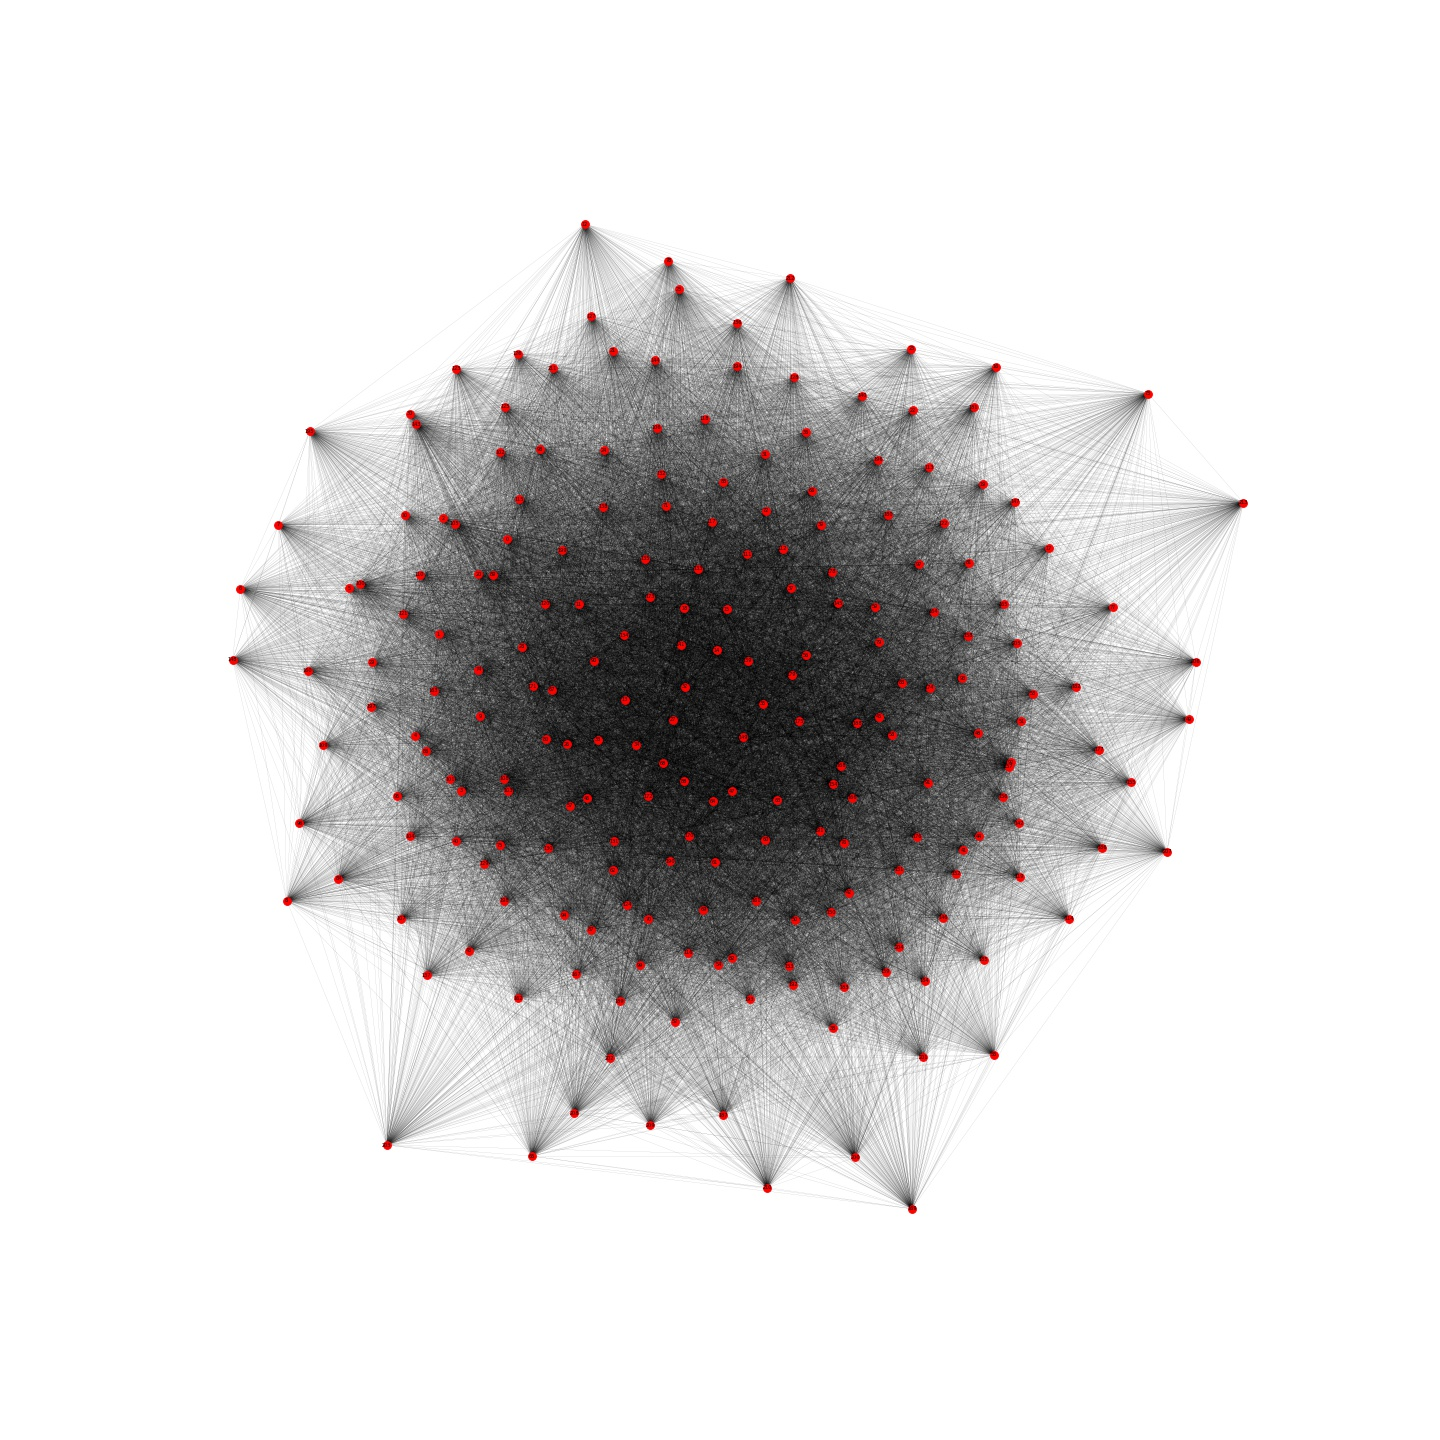
\includegraphics[width=.8\linewidth]{spring.jpg}
\caption{Just to give a taste of the object that we are dealing with: visualization of the functional brain network. Since this is already an overly complicated picture, we don't bother to draw the other two. Each node corresponds to a brain region and edges are defined by functional correlation between  these regions}
\label{fig:network}
\end{figure}

Both the structural and functional network constructions, which generally yield a fully connected and weighted adjacency matrix, from the brain imaging data involve a thresholding of the edge weights ending up loosing structural and functional meaning because we do not have a generally accepted criteria for determining a proper threshold. So, instead of trying to come up with a proper threshold for network construction that may not work for different populations or cognitive conditions, we propose a multiscale framework that models all brain networks generated over every possible threshold and traces the evolution of network changes over different thresholds. This method is going to enable us to capture the information over all weight scales especially the regions of lower edge weights that has been neglected so far due to the ad hoc thresholding methods. So, we are mainly interested in the lower connectivity regions and it has been claimed that these reduced connectivity regions might actually be responsible from resting-state dynamics, cognitive control and correlated network states(cite), so overlooking the activity of these regions may end up ignoring the potential research results.



  In network theory, a k-clique is the subset of nodes in which every node is connected to k-1 others among the subset. A converse to this concept would be fully disconnected set of nodes. However, we are assuming our networks has one connected component. So, a partial converse can be defined as a hole, or a loop, in a network which can be thought of as removing some number of edges from the clique without changing the number of connected components. These regions in the brain networks can be characterized by a low connectivity region meaning that this part of the network does not completely shut down but works in a lower capacity, whereas a region without a hole, consisting of a clique is a stronger connectivity region in which every node of the network compounding the clique considered as engaging in the process of whatever the network does.
  
\begin{figure}%[tbhp]
\centering
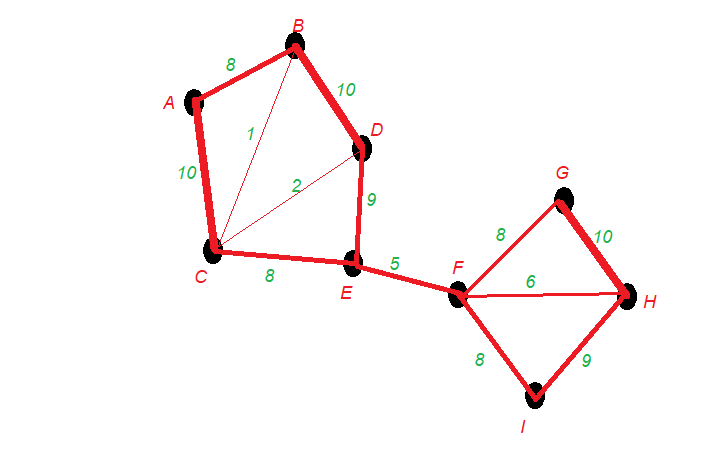
\includegraphics[width=.8\linewidth]{lower_connectivity.png}
\caption{An example of comparisons between lower connectivty regions in a basic weighted network. The hole ABDEC is different from the hole FGHI in terms of depths. The former  loop appears when the all edges with weight 8 is present and dies the edge CD enters the filtration adding up to a total depth of 6. On the other hand, the loop FGHI appear at the same time as ABDEC but closes the edge FH enters the filtration at weight 6 adding up to a total depth of 2}
\label{fig:connectivty}
\end{figure}


\begin{figure*}%[tbhp]
\centering
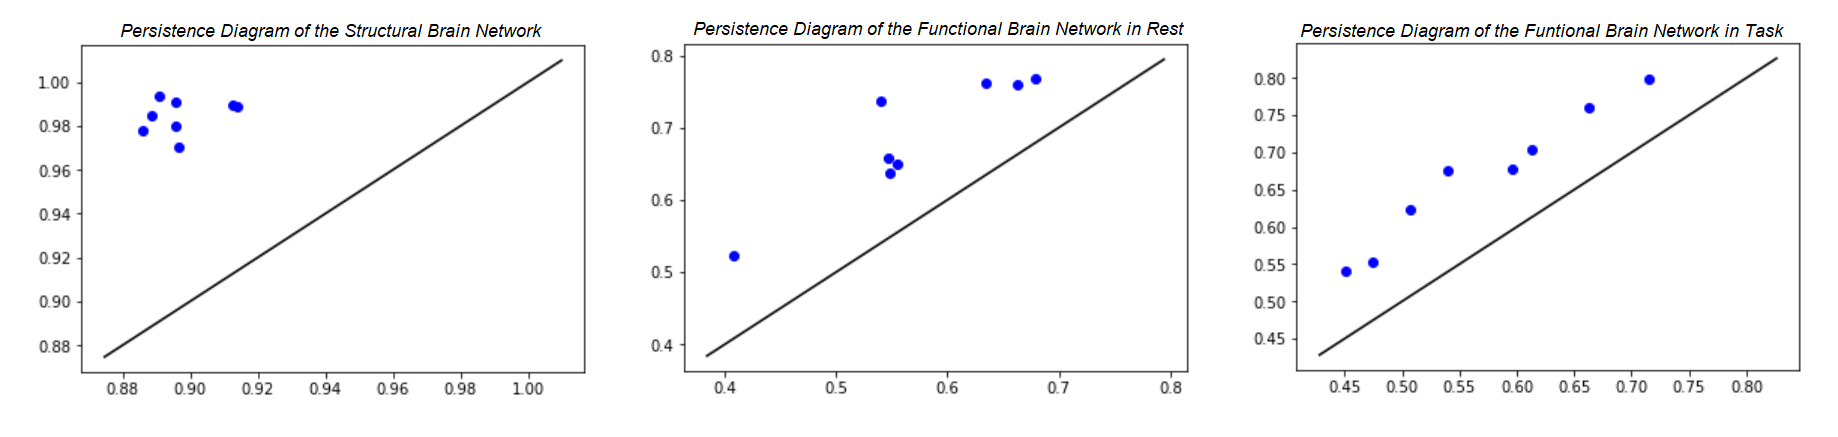
\includegraphics[width=16cm,height=6cm]{peristencediagrams.png}
\caption{Left: Strong edges compounding the loops in the structural brain network comes with strong edges making them a clique, so they don't appear in the persistence diagram. What we see is the weak edges, entering the filtration later on, whose filling edges are absent. Right: loops are appearing at every weight scale; weak edges lack of weaker edges making them a clique as well as strong edges lacking less strong edges making them a clique. Middle: the picture is sort of in the middle of the scale}
\end{figure*}

On the other hand, a loop in an abstract topological space can be characterized algebraically by the homology groups of that space. Homology is a vector space obtained by quotient of the image of a boundary map by the kernel of the following boundary map such that the composition of the boundary maps is trivial. Depending on the dimensions of the boundary maps, the interpretation of homology changes. In the 0-dimensional case, homology counts the connected components of an abstract space. Whereas, in the 1-dimensional case, homology counts loops or 1-dimensional holes and in dimension 2, homology corresponds to the voids enclosed by some volume. It's harder to visualize generic n-dimensional analogues of homology, but rule of thumb is still legit: homology is an algebraic invariant. In the literature, n-th Betti number corresponds to the dimension of the n-th homology which is what we mean by counting the connected components, loops and voids. Given that a network can be constructed via combinatorial structures, so called simplices, every network can be given a topology i.e. every network is a topological object. Therefore, every network is prone to the tools of algebraic topology. So, just like degree, modularity or eigenvalue centrality, homology can be taught of as a network measure whose meaning is slightly less trivial. Yet, the meaning of a loop in the brain network setting is explained in the previous paragraph for reader to build bridges between two areas.

Persistent homology is a recent technique whose applications gained a lot of attention from different research fields over the past decade. Main idea of persistent homology is that building a nested sequence of subspaces, which is called a filtration, that approximates the original data set. Choosing how to build the filtration is like choosing the lenses that one looks at the data set(cite). Different filtration constructions would yield different results and most of the time filtration can be defined via a real valued function. More formally, let $X$ be the original data set we want to examine and $X_{0}\subset X_{1}\subset...\subset X_{N}=X $ be the filtration. Then, one can compute the homology of each individual spaces and keep track of the homological features that persisted in terms of filtration steps.  The main assumption of the persistent homology is that actual signal in the data is going to persist for a long time whereas shorter persistent cycles are likely to be just noise. This approach highlights not only the mesosopic regions of reduced connectivity but also how network properties evolve along the filtration.



\section*{Results}

We start with 14 individuals whose structural brain network is obtained via diffusion imaging and functional brain network in resting state is obtained via BOLD signals. For comparison, we also measure the BOLD signals in a modular arithmetic test and turned it into a functional brain network. Then, we averaged the data among 14 individuals and carry on the analysis with only three networks: structural, functional in rest and functional in task. After the computation of 1st homology generators of each networks, we kept the 8 cycles that persisted most in each of them. Figure 2 shows the persistence diagrams corresponding to each instance. The appearance of the lower connectivity regions throughout the filtration is different in each case. Even though we didn't realize a significant difference in terms of persistence durations of these cycles, in the structural network, we noticed all 8 generators born towards the end of the filtration whereas functional brain network in rest shows a little more linear distribution throughout the filtration. Functional brain network in task demonstrates the most linear distribution meaning that the brain turns into a more organized state during a task engaging different levels of lower connectivity regions i.e. several loops born at different weights with pretty much the same depth. On the other hand, in the structural brain network, holes are tend to born and die around the same weight scale. 

Another interesting observation is that in the structural brain network, we observed a lower mesosopic region of connectivity, a loop, between the left and right hemispheres of the brain. Specifically, there exists a hole whose edges run through the brain region LH/SomMotA and RH/SomMotA consistently whereas other loops we found are going through multiple brain regions. This result might be interpreted as, part of the somatomotor system, region A in particular, is structurally a lower connectivity region given that sensory stimulus can be present any time and brain doesn't shut down this system completely, but it let's it run at the background and ready to operate.

Then, we compare the results from the homological scaffold networks $N'_{Structural}$, $N'_{Rest}$ and $N'_{MOD}$ in terms of the classical network measures. First thing that draw our attention is that no subcortical region was present in both of the functional homological scaffolds i.e. loops doesn't go through the nodes with ids 200-214 which are precisely the subcortical areas  in the brain. However, there is fair amount of subcortical regions contributing to the structural homological scaffold. Furthermore, another interesting similarity between resting state and task state homological scaffolds is that the most in between edges, the highest edge betweenness centrality, are between the brain regions RH/ContB-RH/DorsAttnA and RH/DorsAttnA-RH/DorsAttnB in both of the functional brain networks-in rest and in task. 

We kept going investigating these new networks that has constructed in terms of other network measures. Algebraic connectivity of these 
\begin{table}%[tbhp]
\centering
\caption{Comparison of the algebraic connectivity, transitivity and global efficiency of $N'_{Structural}$, $N'_{Rest}$ and $N'_{Task}$}
\begin{tabular}{lrrr}
Scaffolds & A. Connectivity & Transitivity & Global Efficiency \\
\midrule
1. $N'_{Structural}$ & 0.02353226686 & 0.0769230769 & 0.2331699031 \\
2. $N'_{Rest}$ & 0.09224809273 & 0.1818181818 & 0.4360507246 \\
3. $N'_{Task}$ & 0.02378270622 & 0.1942446043 & 0.4063218390\\
\bottomrule
\end{tabular}

\addtabletext{Comparisons of the network measures based on the information flow}
\end{table}

\section*{Discussion}

\section*{Methods and Materials}

\subsection{Structural and Functional Correlation Dataset} Structural connectivity from 14 individuals obtained via diffusion spectrum imaging(DSI) data and tractography. As a result, 17 systems in each hemisphere further divided into 107 cortical and subcortical regions of interests, making 214 nodes in total.
The empirical resting-state functional connectivity was also obtained from the same 14 subjects by measuring the corresponding fMRI BOLD signals and divided into 214 brain regions for a legit comparison between function and structure. For the task performance, we chose a modular arithmetic test and acquired the functional connectivity matrices in task ($214\times 214$) for every individual again via the correlation between nodal activities on the basis of blood oxygenation level-dependent functional MRI. 

For our analysis, we mainly used the matrices which are averaged along the individuals and carry on the analysis via three networks; structural, functional resting-state and functional task.

\subsection{Persistent Homology as a Lower Connectivity Region Measure}
As we mentioned earlier, homology is a tool to detect loops and persistent homology is a novel application to the real world datasets. In the brain network case, loops in the network has a special meaning: regions of reduced connectivity.

We started by indexing the filtration $X_{0}\subset X_{1}\subset ...\subset X_{n}=X$ by the ranked edge weights in descending order. This will provide the edges with higher weight entering the filtration earlier and edges with lower edge weight later enabling the loop structures to be more significant before they get killed by a 2-cell, or a 3-clique which is nothing but a triangle. So, our construction goes as follows: given that we have a weighted undirected network $N=(V,E,\omega)$, all 0-cells, the set of vertices $V$, are assumed to be having weight $0$, so they are going to be present in the space $X_{0}$. Then, in the first filtration step $X_{1}$, edges with maximum weight $\omega_{max}$ are going to enter the filtration. Then, in $X_{2}$, some edges with weight $\omega<\omega_{max}$ are entering the filtration in order to have $X_{1}\subset X_{2}$ and so on. Finally, the weight of a 2-cell is determined by minimum of it's coboundary so that at each step we'll have a closed 2-skeleton. Persistent homology computation can be reduced to gaussian elimination and can be done by the algorithm given in the original paper(zomoridan) easily. Although, there are several packages in Python and MatLab that computes the persistent homology of a filtration, a good review article can be found (cite), we prefer to use our own(eztda).

A persistence diagram is a scatter of points above the $x=y$ line that demonstrates the birth and death times of the homology generators in a compact fashion. The birth time $\beta_{c}$ represents the filtration index in which that homological feature has appeared and the death time $\gamma_{c}$ represents the filtration index in which the homological feature disappear giving us a total survival time $\pi_{c}=\gamma_{c}-\beta_{c}$ which we call persistence.  The further up a point is from the diagonal, the more meaningful the information that point represents.

\subsection{Homological Scaffolds of the Reduced Connectivity Regions}
After computing the homology generators for the three main networks, we apply a persistence threshold keeping the most persistent 8 cycles in each network. A cycle $g_{c}$ is a chain of edges enclosing a loop in the network. So, to see that which brain regions are contributing to the reduced connectivity of the brain systemwise, we grouped together the 214 nodes in the networks according to the systems and hemispheres that they belong resulting in 34 nodes, 17 in each hemisphere and added the homology generators as edges with weight summed persistence value. More formally, let $N=(V,E,\omega)$ be as before, we constructed a new network $N'=(V',E',\omega^{\pi})$ from the homological information such that $V'=\{v_{i_{k}}|,i=1,..,34, k $ is the number of nodes in each system \} and $E'=\bigcup_{c\in C}g_{c}$ where $C$ is the set of 8 cycles found by the persistent homology computation and the weights are given by:

\begin{align*}
\omega^{\pi}_{e'}=\sum_{g_{c}|e'\in g_{c}}\pi_{g_{c}} \numberthis\\
\end{align*}

We continued our analysis with these three new networks $N'_{structural}, N'_{rest}$ and $N'_{task}$.

\begin{figure*}%[tbhp]
\centering
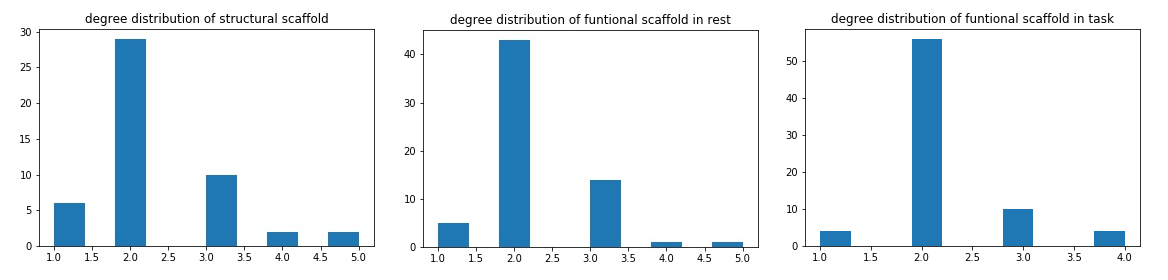
\includegraphics[width=16cm,height=6cm]{degreedists.png}
\caption{Degree distributions of the $N'_{Structural}$, $N'_{Rest}$ and $N'_{MOD}$. Since these networks are consisting of loops i.e. they are union of ring graphs, there shouldn't be any nodes with degree one. However, we know that persistent homology calculation returns the homological information with some noise which are the degree 1 nodes in this case. So, it makes sense that most of the edges have degree two and then degree distribution follows a power law pattern.}
\end{figure*}



\acknow{Please include your acknowledgments here, set in a single paragraph. Please do not include any acknowledgments in the Supporting Information, or anywhere else in the manuscript.}

\subsection*{References}

References should be cited in numerical order as they appear in text; this will be done automatically via bibtex, e.g. \cite{belkin2002using} and \cite{berard1994embedding,coifman2005geometric}. All references should be included in the main manuscript file.



\begin{figure}%[tbhp]
\centering

\includegraphics[width=.8\linewidth]{frog.eps}
\caption{Placeholder image of a frog with a long example caption to show justification setting.}
\label{fig:frog}
\end{figure}


\begin{SCfigure*}[\sidecaptionrelwidth][t]
\centering
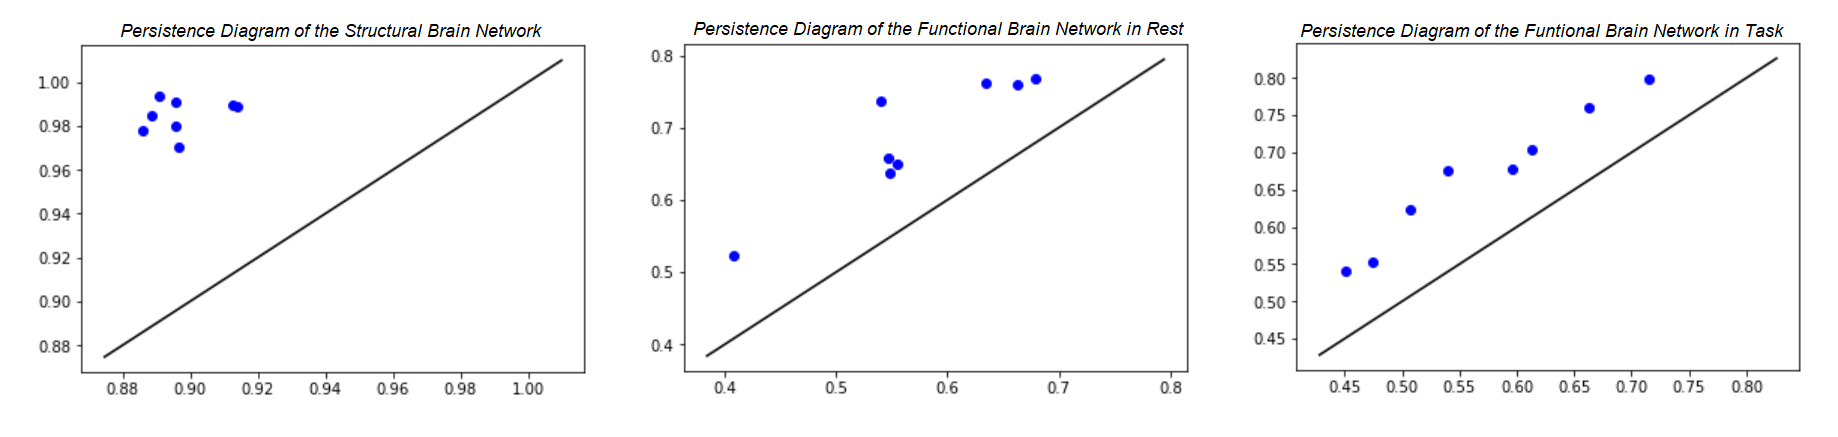
\includegraphics[width=18cm,height=6cm]{peristencediagrams.png}
\caption{This caption would be placed at the side of the figure, rather than below it.}
\end{SCfigure*}


\subsection*{Tables}
In addition to including your tables within this manuscript file, PNAS requires that each table be uploaded to the submission separately as a “Table” file.  Please ensure that each table .tex file contains a preamble, the \verb|\begin{document}| command, and the \verb|\end{document}| command. This is necessary so that the submission system can convert each file to PDF.


\begin{figure*}[bt!]
\begin{align*}
(x+y)^3&=(x+y)(x+y)^2\\
       &=(x+y)(x^2+2xy+y^2) \numberthis \label{eqn:example} \\
       &=x^3+3x^2y+3xy^3+x^3. 
\end{align*}
\end{figure*}


\begin{table}%[tbhp]
\centering
\caption{Comparison of the fitted potential energy surfaces and ab initio benchmark electronic energy calculations}
\begin{tabular}{lrrr}
Species & CBS & CV & G3 \\
\midrule
1. Acetaldehyde & 0.0 & 0.0 & 0.0 \\
2. Vinyl alcohol & 9.1 & 9.6 & 13.5 \\
3. Hydroxyethylidene & 50.8 & 51.2 & 54.0\\
\bottomrule
\end{tabular}

\addtabletext{nomenclature for the TSs refers to the numbered species in the table.}
\end{table}

\acknow{Please include your acknowledgments here, set in a single paragraph. Please do not include any acknowledgments in the Supporting Information, or anywhere else in the manuscript.}

\showacknow{} % Display the acknowledgments section

% Bibliography
\bibliography{pnas-sample}

\end{document}